\iffalse
\documentclass[journal,12pt,twocolumn]{IEEEtran}

\usepackage[utf8]{inputenc}
\usepackage{kvmap}
\usepackage{graphics} 

\usepackage{setspace}
\usepackage{gensymb}

\singlespacing


\usepackage{amsthm}

\usepackage{mathrsfs}
\usepackage{txfonts}
\usepackage{stfloats}
\usepackage{bm}
\usepackage{cite}
\usepackage{cases}
\usepackage{subfig}

\usepackage{longtable}
\usepackage{multirow}

\usepackage{enumitem}
\usepackage{mathtools}
\usepackage{steinmetz}
\usepackage{tikz}
\usepackage{circuitikz}
\usepackage{verbatim}
\usepackage{tfrupee}
\usepackage[breaklinks=true]{hyperref}
\usepackage{graphicx}
\usepackage{tkz-euclide}
\usepackage{float}

\usetikzlibrary{calc,math}
\usepackage{listings}
    \usepackage{color}                                            %%
    \usepackage{array}                                            %%
    \usepackage{longtable}                                        %%
    \usepackage{calc}                                             %%
    \usepackage{multirow}                                         %%
    \usepackage{hhline}                                           %%
    \usepackage{ifthen}                                           %%
    \usepackage{lscape}     
\usepackage{multicol}
\usepackage{chngcntr}

\DeclareMathOperator*{\Res}{Res}

\renewcommand\thesection{\arabic{section}}
\renewcommand\thesubsection{\thesection.\arabic{subsection}}
\renewcommand\thesubsubsection{\thesubsection.\arabic{subsubsection}}

\renewcommand\thesectiondis{\arabic{section}}
\renewcommand\thesubsectiondis{\thesectiondis.\arabic{subsection}}
\renewcommand\thesubsubsectiondis{\thesubsectiondis.\arabic{subsubsection}}


\hyphenation{op-tical net-works semi-conduc-tor}
\def\inputGnumericTable{}                                 %%

\lstset{
%language=C,
frame=single, 
breaklines=true,
columns=fullflexible
}
\begin{document}


\newtheorem{theorem}{Theorem}[section]
\newtheorem{problem}{Problem}
\newtheorem{proposition}{Proposition}[section]
\newtheorem{lemma}{Lemma}[section]
\newtheorem{corollary}[theorem]{Corollary}
\newtheorem{example}{Example}[section]
\newtheorem{definition}[problem]{Definition}

\newcommand{\BEQA}{\begin{eqnarray}}
\newcommand{\EEQA}{\end{eqnarray}}
\newcommand{\define}{\stackrel{\triangle}{=}}
\newcommand\hlight[1]{\tikz[overlay, remember picture,baseline=-\the\dimexpr\fontdimen22\textfont2\relax]\node[rectangle,fill=blue!50,rounded corners,fill opacity = 0.2,draw,thick,text opacity =1] {$#1$};}
\bibliographystyle{IEEEtran}
\providecommand{\mbf}{\mathbf}
\providecommand{\pr}[1]{\ensuremath{\Pr\left(#1\right)}}
\providecommand{\qfunc}[1]{\ensuremath{Q\left(#1\right)}}
\providecommand{\sbrak}[1]{\ensuremath{{}\left[#1\right]}}
\providecommand{\lsbrak}[1]{\ensuremath{{}\left[#1\right.}}
\providecommand{\rsbrak}[1]{\ensuremath{{}\left.#1\right]}}
\providecommand{\brak}[1]{\ensuremath{\left(#1\right)}}
\providecommand{\lbrak}[1]{\ensuremath{\left(#1\right.}}
\providecommand{\rbrak}[1]{\ensuremath{\left.#1\right)}}
\providecommand{\cbrak}[1]{\ensuremath{\left\{#1\right\}}}
\providecommand{\lcbrak}[1]{\ensuremath{\left\{#1\right.}}
\providecommand{\rcbrak}[1]{\ensuremath{\left.#1\right\}}}
\theoremstyle{remark}
\newtheorem{rem}{Remark}
\newcommand{\sgn}{\mathop{\mathrm{sgn}}}
\providecommand{\abs}[1]{\left\vert#1\right\vert}
\providecommand{\res}[1]{\Res\displaylimits_{#1}} 
\providecommand{\norm}[1]{$\left\lVert#1\right\rVert$}
%\providecommand{\norm}[1]{\lVert#1\rVert}
\providecommand{\mtx}[1]{\mathbf{#1}}
\providecommand{\mean}[1]{E\left[ #1 \right]}
\providecommand{\fourier}{\overset{\mathcal{F}}{ \rightleftharpoons}}
%\providecommand{\hilbert}{\overset{\mathcal{H}}{ \rightleftharpoons}}
\providecommand{\system}{\overset{\mathcal{H}}{ \longleftrightarrow}}
	%\newcommand{\solution}[2]{\textbf{Solution:}{#1}}
\newcommand{\solution}{\noindent \textbf{Solution: }}
\newcommand{\cosec}{\,\text{cosec}\,}
\providecommand{\dec}[2]{\ensuremath{\overset{#1}{\underset{#2}{\gtrless}}}}
\newcommand{\myvec}[1]{\ensuremath{\begin{pmatrix}#1\end{pmatrix}}}
\newcommand{\mydet}[1]{\ensuremath{\begin{vmatrix}#1\end{vmatrix}}}
\numberwithin{equation}{subsection}
\makeatletter
\@addtoreset{figure}{problem}
\makeatother
\let\StandardTheFigure\thefigure
\let\vec\mathbf
\renewcommand{\thefigure}{\theproblem}
\def\putbox#1#2#3{\makebox[0in][l]{\makebox[#1][l]{}\raisebox{\baselineskip}[0in][0in]{\raisebox{#2}[0in][0in]{#3}}}}
     \def\rightbox#1{\makebox[0in][r]{#1}}
     \def\centbox#1{\makebox[0in]{#1}}
     \def\topbox#1{\raisebox{-\baselineskip}[0in][0in]{#1}}
     \def\midbox#1{\raisebox{-0.5\baselineskip}[0in][0in]{#1}}
\vspace{3cm}
\title{\textbf{Matrix Assignment - Circle} }
\author{Surabhi Seetha}
\maketitle
\newpage
\bigskip
\renewcommand{\thefigure}{\theenumi}
\renewcommand{\thetable}{\theenumi}
Get Python code for the figure from 
\begin{lstlisting}
https://github.com/SurabhiSeetha/Fwciith2022/tree/main/Assignment%201/codes/src
\end{lstlisting}
Get LaTex code from
\begin{lstlisting}
https://github.com/SurabhiSeetha/Fwciith2022/tree/main/avr%20gcc
\end{lstlisting}
%
\section{Question-Class 10, Exercise 11.2, Q(5)}
\textbf{
\fi
	Draw a line segment $AB$ of length 8cm. Taking $\vec{A}$ as centre, draw a circle of radius 4cm and taking $\vec{B}$ as centre, draw another circle of radius 3cm. Construct tangents to each circle from the centre of the circle.
	\\
	\solution See Fig. 
		\ref{fig:10/11/2/5}.
	\begin{figure}[!h]
		\centering
 \includegraphics[width=\columnwidth]{chapters/10/11/2/5/figs/cir.png}
		\caption{}
		\label{fig:10/11/2/5}
  	\end{figure}
	\iffalse
} \\


\centering
\includegraphics[width=0.45\textwidth]{cir.png}
Figure- Circles A and B with tangents P1,P2,Q1,Q2

\section{Construction}
\vspace{0.25cm}
\raggedright
A circle with radius 4cm and another circle with radius 3cm are taken and their tangents are drawn with their point of contacts as P1,P2,Q1 and Q2 and their construction is done with the help of $\theta$ and $\alpha$ angles as shown in the table below.\\
\centering
\begin{tabular}{|c|c|c|}
\hline
\textbf{Symbol} & \textbf{Value} & \textbf{Description} \\
\hline
$r_1$ & 4cm & radius\\
\hline
$r_2$ & 3cm & radius\\
\hline
O & $\myvec{0\\0}$ & Center O\\
\hline
d & 8cm & Distance OC\\
\hline
$e_1$ & $\myvec{1\\0}$ &  Unit Vector\\
\hline
C & d x $e_1$ & Centre C\\
\hline
$\theta$ & $\angle P_1OC$ & Angle $P_1OC$\\
\hline
$\alpha$ & $\angle Q_1OC$ & Angle $Q_1OC$\\
\hline
t & d $cos\alpha$ & $OQ_1$ \\
\hline
$P_1$ & $r_1$ $\myvec{cos\theta\\ sin\theta}$ & P.O.C \\
\hline
$P_2$ & $r_1$ $\myvec{cos\theta\\ -sin\theta}$ & P.O.C \\
\hline
$Q_1$ & t $\myvec{cos\alpha\\ sin\alpha}$ & P.O.C \\
\hline
$Q_2$ & t $\myvec{cos\alpha\\ -sin\alpha}$ & P.O.C \\
\hline

\end{tabular}

\section{Solution}
\raggedright{\subsection{Part-1:}}
Consider the circle A of radius 4cm and points O and C each at a distance 8cm from the centre. Two tangents can be drawn from point O onto the circle B with point of contacts Q1,Q2 and other two tangents from point C onto the circle A with the point of contacts P1,P2.\\
\vspace{0.25cm}
\raggedright{The point of intersection of line:}\\
\begin{align}
L:\textbf{x}=\textbf{q}+\mu \textbf{m}           
\label{eq1}
\end{align}
\raggedright{with the conic section:}\\
\begin{align}
\textbf{x}^T\textbf{Vx}+2\textbf{u}^T\textbf{x}+f=0     
\label{eq2}
\end{align}
\raggedright{is given by-}\\
\begin{align}
\vec{x_i}=\vec{q}+\mu_i\vec{m}             
\label{eq3}
\end{align}
\raggedright{where,}\\
$\mu_i=\frac{1}{\vec{m}^T\vec{Vm}}(-\vec{m}^T(\vec{Vq}+\vec{u})$\\ 
\begin{align}
\pm\sqrt{(\vec{m}^T(\vec{Vq+u}))^2-(\vec{q}^T+2\vec{u}^T\vec{q}+f)(\vec{m}^T\vec{Vm})}                 
\label{eq4}
\end{align}
\vspace{0.25cm}
\raggedright{If the line L touches the conic at exactly one point q}\\
where q is the point of origin(0,0) which is A\\
\begin{align}
\vec{m}^T(\vec{Vq}+\vec{u}=0)                 
\label{eq5}
\end{align}

\vspace{0.25cm}
\raggedright
In this case,the conic intercept has exactly one root Hence,\\
\vspace{0.25cm}
\begin{align}
[\vec{m}^T(\vec{Vq}+\vec{u})]^2-(\vec{m}^T\vec{Vm})(\vec{q}^T\vec{Vq}+2\vec{u}^T\vec{q}+f)=0    
\label{eq6}
\end{align}
\raggedright\vspace{0.25cm}
So,comparing the equation of our conic $x^2+y^2=4^2$ with the general Equation of a circle:\\
\vspace{0.25cm}
\centering{$Ax^2+Bxy+Cy^2+Fx+Gy+f=0$}\\
\centering\vspace{0.15cm}{$x^2+y^2-16=0$}\\
\raggedright{we get,}\\
\vspace{0.15cm}
\centering{$\vec{V}=\myvec{A&\frac{B}{2} \\\\ \frac{B}{2}&C}$}
\hspace{1.5cm}$\vec{u}=\myvec{\frac{F}{2} \\\\ \frac{G}{2}}$\\
\vspace{0.25cm}
\hspace{0.3cm}{$\vec{V}=\myvec{1&0 \\\\ 0&1}$}
\hspace{1.5cm} $\vec{u}=\myvec{0 \\ 0}$\\
\vspace{0.25cm}
\raggedright
Substituting the above values in eq.\eqref{eq2} we get,\\
\vspace{0.25cm}
\begin{align}
\vec{x}^T\vec{Vx}+2(0\hspace{0.2cm}0)\vec{x}+4=0        
\label{eq7}
\end{align}
\vspace{0.25cm}
\raggedright{Let us consider the direction vector of L as m}\\
\vspace{0.25cm}
\begin{align}
\vec{m}=\myvec{1 \\ \lambda}    
\label{eq8}
\end{align}
\raggedright{and q be the pont A,}\\
\begin{align}
\vec{q}=\myvec{8 \\ 0}        
\label{eq9}
\end{align}
\raggedright{Substituting eq. \eqref{eq7}, \eqref{eq8} and \eqref{eq9} in Eq.\eqref{eq6} we get,}\\
\vspace{0.25cm}
\centering{$[\vec{m}^T(\vec{Iq})]^2-(\vec{m}^T\vec{Im})(\vec{q}^T\vec{Iq}+(-16))=0$}\\
\vspace{0.3cm}
\begin{align}
[\myvec{1&\lambda} \myvec{8 \\ 0}]^2-(\myvec{1&\lambda} \myvec{1 \\ \lambda})(\myvec{8&0}\myvec{8 \\ 0}-16)=0    
\label{eq10}
\end{align}
\vspace{0.25cm}
\centering{$8^2-(1+\lambda^2)(64-16)=0$}\\
\vspace{0.25cm}
$64-(1+\lambda^2)(48)=0$\\
\vspace{0.25cm}
$(1+\lambda^2)=\frac{64}{48}$\\
\vspace{0.25cm}
\begin{align}
\vec{\lambda}=\pm\frac{1}{\sqrt{3}}         
\label{eq11}
\end{align}
\raggedright{That is,}\\
\vspace{0.25cm}
\begin{align}
\vec{m}=\myvec{1  \\ \pm{\frac{1}{\sqrt{3}}}}         
\label{eq12}
\end{align}
\raggedright{from \eqref{eq4} and \eqref{eq6}}\\
\vspace{0.25cm}
\begin{align}
\mu_i=\frac{1}{\vec{m}^T\vec{Vm}}(\vec{-m}^T(\vec{Vq}+\vec{u})) 
\label{eq13}
\end{align}
\vspace{0.25cm}
$ \mu_i = \frac{1}{\myvec{1 \\ \frac{1}{\sqrt{3}}} I \myvec{1 & \frac{1}{\sqrt{3}}}} (-(1 \pm\frac{1}{\sqrt{3}}\myvec{8 \\ 0})$\\
\vspace{0.25cm}
$\mu_i=\frac{1}{1+\frac{1}{3}}(-8)$\\
\vspace{0.25cm}
\begin{align}
\mu_i=-6
\label{eq14}
\end{align}
\vspace{0.25cm}
\raggedright{Now eq. \eqref{eq3} becomes,}\\
\vspace{0.25cm}
\centering
\begin{align}
\myvec{x \\ y} = \myvec{8\\0} + (-6)  \myvec{1 \\ \pm \frac{1}{\sqrt{3}}}
\label{eq15}
\end{align}  
\vspace{0.25cm}
\begin{align}
\myvec{x \\ y} = \myvec{8\\0} + \myvec{-6 \\ \pm \frac{6}{\sqrt{3}}}
\label{eq16}
\end{align}  
\vspace{0.25cm}
\begin{align}
\myvec{x \\ y} = \myvec{2 \\ \pm \frac{6}{\sqrt{3}}}
\label{eq17}
\end{align}  
\vspace{0.25cm}
\raggedright
Therefore,\\
\vspace{0.25cm}
\centering
$ \vec{P_1} = \myvec{2 \\ \frac{6}{\sqrt{3}}} = \myvec{2\\3.464} $\\
\vspace{0.25cm}
$ \vec{P_2} = \myvec{2 \\ -\frac{6}{\sqrt{3}}} = \myvec{2\\-3.464} $\\
\raggedright{\subsection{Part-2:}}
Now for another circle B of radius 3cm which has its tangents drawn from circle A onto B with the point of contacts namely $Q_1$ and $Q_2$.\\
\vspace{0.25cm}
Let us consider the same line and conic equations as in Part 1. The line L touches the conic at exactly one point q.\\
\vspace{0.25cm}
\centering
\begin{align}
\vec{m}^T (\vec{Vq} + \vec{u}) = 0  
\label{eq18}
\end{align}
\vspace{0.25cm}
\raggedright
Hence,\\
\vspace{0.25cm}
\centering
\begin{align}
[ \vec{m}^T (\vec{Vq} + \vec{u}) ]^2 -(\vec{m}^T \vec{Vm})(\vec{q}^T \vec{Vq} + 2\vec{u}^T \vec{q} + f) = 0 
\label{eq19}
\end{align}
\vspace{0.25cm}
\raggedright
The equation of conic is,\\
\vspace{0.25cm}
\centering
$ (x-8)^2 + y^2 = 3^2 $\\
\vspace{0.25cm}
$ x^2 + 64 -16x + y^2 - 9 = 0$ \\
\vspace{0.25cm}
$ x^2 - 16x + y^2 + 55 = 0 $ \\
\vspace{0.25cm}
\raggedright
Comparing it with general Eq. of a circle\\
\vspace{0.25cm}
\centering
$ A x^2 + Bxy + C y^2 + Fx + Gy + f = 0 $\\
\vspace{0.25cm}
\raggedright
We get,\\
\vspace{0.25cm}
\centering{$\vec{V}=\myvec{A&\frac{B}{2} \\\\ \frac{B}{2}&C}$}
\hspace{1.5cm}$\vec{u}=\myvec{\frac{F}{2} \\\\ \frac{G}{2}}$\\
\vspace{0.25cm}
\hspace{0.3cm}{$\vec{V}=\myvec{1&0 \\\\ 0&1}$}
\hspace{1.25cm} $\vec{u}=\myvec{-8 \\\\ 0}$\\
\vspace{0.25cm}
\raggedright
Now Eq. \eqref{eq2} can be written as,\\
\vspace{0.25cm}
\centering
\begin{align}
\vec{x}^T \myvec{1&0\\0&1} x + 2 \myvec{-8&0} \vec{x} + 3 = 0 
\label{eq20}
\end{align}
\vspace{0.25cm}
\raggedright{Let us consider the direction vector of \textbf{L} as m}\\
\vspace{0.25cm}
\begin{align}
\vec{m}=\myvec{1 \\ \lambda}     
\label{eq21}
\end{align}
\raggedright{and q be the pont A,}\\
\begin{align}
\vec{q}=\myvec{0 \\ 0} 
\label{eq22}
\end{align}
\raggedright{Substituting the above values in eq. \eqref{eq19} we get,}\\
\vspace{0.25cm}
\centering
$ [ \vec{m}^T (\vec{Vq} + \vec{u}) ]^2 -(\vec{m}^T \vec{Vm})(\vec{q}^T \vec{Vq} + 2\vec{u}^T \vec{q} + f) = 0$ \\
\vspace{0.25cm}
$ [ \myvec{1 & \lambda} [I \myvec{0\\0} + \myvec{-8 \\ 0}]]^2 - ( \myvec{1&\lambda} I \myvec{1\\ \lambda}) (55) = 0 $ \\
\vspace{0.25cm}
$ [ \myvec{1 & \lambda} \myvec{-8 \\ 0}]^2 - (1 + \lambda^2) (55) = 0 $ \\
\vspace{0.25cm}
$ 64 - ( 1 + \lambda^2 ) 55 = 0 $\\
\vspace{0.25cm}
$ 64 - 55 - 55\lambda^2 = 0 $ \\
\vspace{0.25cm}
$ \lambda^2 = \frac{9}{55}$ \\
\vspace{0.25cm}
\begin{align}
\lambda = \pm \frac{3}{\sqrt{55}} = \pm 0.4
\label{eq23}
\end{align}
\vspace{0.25cm}
\raggedright
Now,\\
\vspace{0.1cm}
\centering
$ \vec{m} = \myvec{1 \\ \pm0.4045} $ \\
\vspace{0.25cm}
\raggedright
From eq. \eqref{eq4} and \eqref{eq6},\\
\vspace{0.25cm}
\centering
$\mu_i=\frac{1}{\vec{m}^T\vec{Vm}}(\vec{-m}^T(\vec{Vq}+\vec{u}))$ \\
\vspace{0.25cm}
$ \mu_i = \frac{1}{\myvec{1\\0.4045} \hspace{0.1cm} I \hspace{0.1cm} \myvec{1 & 0.4045}} (- \myvec{1 & 0.4045} ( I \myvec{0\\0} + \myvec{-8\\0} ) $ \\
\vspace{0.25cm}
\raggedright
\hspace{1cm} $ = \frac{1}{1 + 0.163} ( - \myvec{1 & 0.4045} \myvec{-8 \\ 0} )$ \\
\vspace{0.25cm}
\hspace{1cm} $ = \frac{1}{1.163} \hspace{0.25cm} \times \hspace{0.25cm} 8 $ \\
\vspace{0.25cm}
Therefore,\\
\vspace{0.1cm}
\centering
$ \vec{\mu_i} = \frac{8}{1.163} = 6.875 $ \\
\vspace{0.25cm}
\raggedright
Now eq. \eqref{eq3} becomes,\\
\centering
\vspace{0.1cm}
$ \vec{x_i} = \vec{q} + \mu_i \vec{m} $ \\
\vspace{0.25cm}
$ = \myvec{0\\0} + 6.875 \myvec{1\\ \pm 0.4045} $ \\
\vspace{0.25cm}
\centering
$ x_i = \myvec{x\\y} = \myvec{6.875 \\ \pm 2.7810} $ \\
\vspace{0.25cm}
\raggedright
Therefore,\\
\vspace{0.25cm}
\centering
$ \vec{Q_1} = \myvec{6.875 \\ 2.7810} $ \\
\vspace{0.25cm}
$ \vec{Q_2} = \myvec{6.875 \\ -2.7810} $ \\
\raggedright
\vspace{0.5cm}
Therefore, we have solved and gained the values of four point of contacts P1,P2,Q1,Q2 for two circles of radius 4cm and 3cm.\\
\end{document}
Footer
\fi
